\documentclass[english, 11 pt, class=article, crop=false]{standalone}
\usepackage[T1]{fontenc}
%\renewcommand*\familydefault{\sfdefault} % For dyslexia-friendly text
\usepackage{lmodern} % load a font with all the characters
\usepackage{geometry}
\geometry{verbose,paperwidth=16.1 cm, paperheight=24 cm, inner=2.3cm, outer=1.8 cm, bmargin=2cm, tmargin=1.8cm}
\setlength{\parindent}{0bp}
\usepackage{import}
\usepackage[subpreambles=false]{standalone}
\usepackage{amsmath}
\usepackage{amssymb}
\usepackage{esint}
\usepackage{babel}
\usepackage{tabu}
\makeatother
\makeatletter

\usepackage{titlesec}
\usepackage{ragged2e}
\RaggedRight
\raggedbottom
\frenchspacing

% Norwegian names of figures, chapters, parts and content
\addto\captionsenglish{\renewcommand{\figurename}{Figur}}
\makeatletter
\addto\captionsenglish{\renewcommand{\chaptername}{Kapittel}}
\addto\captionsenglish{\renewcommand{\partname}{Del}}


\usepackage{graphicx}
\usepackage{float}
\usepackage{subfig}
\usepackage{placeins}
\usepackage{cancel}
\usepackage{framed}
\usepackage{wrapfig}
\usepackage[subfigure]{tocloft}
\usepackage[font=footnotesize,labelfont=sl]{caption} % Figure caption
\usepackage{bm}
\usepackage[dvipsnames, table]{xcolor}
\definecolor{shadecolor}{rgb}{0.105469, 0.613281, 1}
\colorlet{shadecolor}{Emerald!15} 
\usepackage{icomma}
\makeatother
\usepackage[many]{tcolorbox}
\usepackage{multicol}
\usepackage{stackengine}

\usepackage{esvect} %For vectors with capital letters

% For tabular
\usepackage{array}
\usepackage{multirow}
\usepackage{longtable} %breakable table

% Ligningsreferanser
\usepackage{mathtools}
\mathtoolsset{showonlyrefs}

% index
\usepackage{imakeidx}
\makeindex[title=Indeks]

%Footnote:
\usepackage[bottom, hang, flushmargin]{footmisc}
\usepackage{perpage} 
\MakePerPage{footnote}
\addtolength{\footnotesep}{2mm}
\renewcommand{\thefootnote}{\arabic{footnote}}
\renewcommand\footnoterule{\rule{\linewidth}{0.4pt}}
\renewcommand{\thempfootnote}{\arabic{mpfootnote}}

%colors
\definecolor{c1}{cmyk}{0,0.5,1,0}
\definecolor{c2}{cmyk}{1,0.25,1,0}
\definecolor{n3}{cmyk}{1,0.,1,0}
\definecolor{neg}{cmyk}{1,0.,0.,0}

% Lister med bokstavar
\usepackage[inline]{enumitem}

\newcounter{rg}
\numberwithin{rg}{chapter}
\newcommand{\reg}[2][]{\begin{tcolorbox}[boxrule=0.3 mm,arc=0mm,colback=blue!3] {\refstepcounter{rg}\phantomsection \large \textbf{\therg \;#1} \vspace{5 pt}}\newline #2  \end{tcolorbox}\vspace{-5pt}}

\newcommand\alg[1]{\begin{align} #1 \end{align}}

\newcommand\eks[2][]{\begin{tcolorbox}[boxrule=0.3 mm,arc=0mm,enhanced jigsaw,breakable,colback=green!3] {\large \textbf{Eksempel #1} \vspace{5 pt}\\} #2 \end{tcolorbox}\vspace{-5pt} }

\newcommand{\st}[1]{\begin{tcolorbox}[boxrule=0.0 mm,arc=0mm,enhanced jigsaw,breakable,colback=yellow!12]{ #1} \end{tcolorbox}}

\newcommand{\spr}[1]{\begin{tcolorbox}[boxrule=0.3 mm,arc=0mm,enhanced jigsaw,breakable,colback=yellow!7] {\large \textbf{Språkboksen} \vspace{5 pt}\\} #1 \end{tcolorbox}\vspace{-5pt} }

\newcommand{\sym}[1]{\colorbox{blue!15}{#1}}

\newcommand{\info}[2]{\begin{tcolorbox}[boxrule=0.3 mm,arc=0mm,enhanced jigsaw,breakable,colback=cyan!6] {\large \textbf{#1} \vspace{5 pt}\\} #2 \end{tcolorbox}\vspace{-5pt} }

\newcommand\algv[1]{\vspace{-11 pt}\begin{align*} #1 \end{align*}}

\newcommand{\regv}{\vspace{5pt}}
\newcommand{\mer}{\textsl{Merk}: }
\newcommand{\mers}[1]{{\footnotesize \mer #1}}
\newcommand\vsk{\vspace{11pt}}
\newcommand\vs{\vspace{-11pt}}
\newcommand\vsb{\vspace{-16pt}}
\newcommand\sv{\vsk \textbf{Svar} \vspace{4 pt}\\}
\newcommand\br{\\[5 pt]}
\newcommand{\figp}[1]{../fig/#1}
\newcommand\algvv[1]{\vs\vs\begin{align*} #1 \end{align*}}
\newcommand{\y}[1]{$ {#1} $}
\newcommand{\os}{\\[5 pt]}
\newcommand{\prbxl}[2]{
\parbox[l][][l]{#1\linewidth}{#2
	}}
\newcommand{\prbxr}[2]{\parbox[r][][l]{#1\linewidth}{
		\setlength{\abovedisplayskip}{5pt}
		\setlength{\belowdisplayskip}{5pt}	
		\setlength{\abovedisplayshortskip}{0pt}
		\setlength{\belowdisplayshortskip}{0pt} 
		\begin{shaded}
			\footnotesize	#2 \end{shaded}}}

\renewcommand{\cfttoctitlefont}{\Large\bfseries}
\setlength{\cftaftertoctitleskip}{0 pt}
\setlength{\cftbeforetoctitleskip}{0 pt}

\newcommand{\bs}{\\[3pt]}
\newcommand{\vn}{\\[6pt]}
\newcommand{\fig}[1]{\begin{figure}
		\centering
		\includegraphics[]{\figp{#1}}
\end{figure}}

\newcommand{\figc}[2]{\begin{figure}
		\centering
		\includegraphics[]{\figp{#1}}
		\caption{#2}
\end{figure}}

\newcommand{\sectionbreak}{\clearpage} % New page on each section

\newcommand{\nn}[1]{
\begin{equation}
	#1
\end{equation}
}

% Equation comments
\newcommand{\cm}[1]{\llap{\color{blue} #1}}

\newcommand\fork[2]{\begin{tcolorbox}[boxrule=0.3 mm,arc=0mm,enhanced jigsaw,breakable,colback=yellow!7] {\large \textbf{#1 (forklaring)} \vspace{5 pt}\\} #2 \end{tcolorbox}\vspace{-5pt} }
 
%colors
\newcommand{\colr}[1]{{\color{red} #1}}
\newcommand{\colb}[1]{{\color{blue} #1}}
\newcommand{\colo}[1]{{\color{orange} #1}}
\newcommand{\colc}[1]{{\color{cyan} #1}}
\definecolor{projectgreen}{cmyk}{100,0,100,0}
\newcommand{\colg}[1]{{\color{projectgreen} #1}}

% Methods
\newcommand{\metode}[2]{
	\textsl{#1} \\[-8pt]
	\rule{#2}{0.75pt}
}

%Opg
\newcommand{\abc}[1]{
	\begin{enumerate}[label=\alph*),leftmargin=18pt]
		#1
	\end{enumerate}
}
\newcommand{\abcs}[2]{
	\begin{enumerate}[label=\alph*),start=#1,leftmargin=18pt]
		#2
	\end{enumerate}
}
\newcommand{\abcn}[1]{
	\begin{enumerate}[label=\arabic*),leftmargin=18pt]
		#1
	\end{enumerate}
}
\newcommand{\abch}[1]{
	\hspace{-2pt}	\begin{enumerate*}[label=\alph*), itemjoin=\hspace{1cm}]
		#1
	\end{enumerate*}
}
\newcommand{\abchs}[2]{
	\hspace{-2pt}	\begin{enumerate*}[label=\alph*), itemjoin=\hspace{1cm}, start=#1]
		#2
	\end{enumerate*}
}

% Oppgaver
\newcommand{\opgt}{\phantomsection \addcontentsline{toc}{section}{Oppgaver} \section*{Oppgaver for kapittel \thechapter}\vs \setcounter{section}{1}}
\newcounter{opg}
\numberwithin{opg}{section}
\newcommand{\op}[1]{\vspace{15pt} \refstepcounter{opg}\large \textbf{\color{blue}\theopg} \vspace{2 pt} \label{#1} \\}
\newcommand{\ekspop}[1]{\vsk\textbf{Gruble \thechapter.#1}\vspace{2 pt} \\}
\newcommand{\nes}{\stepcounter{section}
	\setcounter{opg}{0}}
\newcommand{\opr}[1]{\vspace{3pt}\textbf{\ref{#1}}}
\newcommand{\oeks}[1]{\begin{tcolorbox}[boxrule=0.3 mm,arc=0mm,colback=white]
		\textit{Eksempel: } #1	  
\end{tcolorbox}}
\newcommand\opgeks[2][]{\begin{tcolorbox}[boxrule=0.1 mm,arc=0mm,enhanced jigsaw,breakable,colback=white] {\footnotesize \textbf{Eksempel #1} \\} \footnotesize #2 \end{tcolorbox}\vspace{-5pt} }
\newcommand{\rknut}{
Rekn ut.
}

%License
\newcommand{\lic}{\textit{Matematikken sine byggesteinar by Sindre Sogge Heggen is licensed under CC BY-NC-SA 4.0. To view a copy of this license, visit\\ 
		\net{http://creativecommons.org/licenses/by-nc-sa/4.0/}{http://creativecommons.org/licenses/by-nc-sa/4.0/}}}

%referances
\newcommand{\net}[2]{{\color{blue}\href{#1}{#2}}}
\newcommand{\hrs}[2]{\hyperref[#1]{\color{blue}\textsl{#2 \ref*{#1}}}}
\newcommand{\rref}[1]{\hrs{#1}{regel}}
\newcommand{\refkap}[1]{\hrs{#1}{kapittel}}
\newcommand{\refsec}[1]{\hrs{#1}{seksjon}}

\newcommand{\mb}{\net{https://sindrsh.github.io/FirstPrinciplesOfMath/}{MB}}


%line to seperate examples
\newcommand{\linje}{\rule{\linewidth}{1pt} }

\usepackage{datetime2}
%%\usepackage{sansmathfonts} for dyslexia-friendly math
\usepackage[]{hyperref}


\newcommand{\note}{Merk}
\newcommand{\notesm}[1]{{\footnotesize \textsl{\note:} #1}}
\newcommand{\ekstitle}{Eksempel }
\newcommand{\sprtitle}{Språkboksen}
\newcommand{\expl}{forklaring}

\newcommand{\vedlegg}[1]{\refstepcounter{vedl}\section*{Vedlegg \thevedl: #1}  \setcounter{vedleq}{0}}

\newcommand\sv{\vsk \textbf{Svar} \vspace{4 pt}\\}

%references
\newcommand{\reftab}[1]{\hrs{#1}{tabell}}
\newcommand{\rref}[1]{\hrs{#1}{regel}}
\newcommand{\dref}[1]{\hrs{#1}{definisjon}}
\newcommand{\refkap}[1]{\hrs{#1}{kapittel}}
\newcommand{\refsec}[1]{\hrs{#1}{seksjon}}
\newcommand{\refdsec}[1]{\hrs{#1}{delseksjon}}
\newcommand{\refved}[1]{\hrs{#1}{vedlegg}}
\newcommand{\eksref}[1]{\textsl{#1}}
\newcommand\fref[2][]{\hyperref[#2]{\textsl{figur \ref*{#2}#1}}}
\newcommand{\refop}[1]{{\color{blue}Oppgave \ref{#1}}}
\newcommand{\refops}[1]{{\color{blue}oppgave \ref{#1}}}
\newcommand{\refgrubs}[1]{{\color{blue}gruble \ref{#1}}}

\newcommand{\openmathser}{\openmath\,-\,serien}

% Exercises
\newcommand{\opgt}{\newpage \phantomsection \addcontentsline{toc}{section}{Oppgaver} \section*{Oppgaver for kapittel \thechapter}\vs \setcounter{section}{1}}


% Sequences and series
\newcommand{\sumarrek}{Summen av en aritmetisk rekke}
\newcommand{\sumgerek}{Summen av en geometrisk rekke}
\newcommand{\regnregsum}{Regneregler for summetegnet}

% Trigonometry
\newcommand{\sincoskomb}{Sinus og cosinus kombinert}
\newcommand{\cosfunk}{Cosinusfunksjonen}
\newcommand{\trid}{Trigonometriske identiteter}
\newcommand{\deravtri}{Den deriverte av de trigonometriske funksjonene}
% Solutions manual
\newcommand{\selos}{Se løsningsforslag.}
\newcommand{\se}[1]{Se eksempel på side \pageref{#1}}

%Vectors
\newcommand{\parvek}{Parallelle vektorer}
\newcommand{\vekpro}{Vektorproduktet}
\newcommand{\vekproarvol}{Vektorproduktet som areal og volum}


% 3D geometries
\newcommand{\linrom}{Linje i rommet}
\newcommand{\avstplnpkt}{Avstand mellom punkt og plan}


% Integral
\newcommand{\bestminten}{Bestemt integral I}
\newcommand{\anfundteo}{Analysens fundamentalteorem}
\newcommand{\intuf}{Integralet av utvalge funksjoner}
\newcommand{\bytvar}{Bytte av variabel}
\newcommand{\intvol}{Integral som volum}
\newcommand{\andordlindif}{Andre ordens lineære differensialligninger}


\begin{document}
\section{Addisjon}

\subsubsection{Oppstilling}
Denne metoden baserer seg på plassverdisystemet, der man trinnvis regner ut summen av enerne, tierne, hundrene, og så videre
\begin{center}
	\parbox{0.3\linewidth}{
\eks[1]{
	\begin{figure}
		\centering
		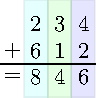
\includegraphics[]{rekfig/plus1}
	\end{figure}
}
}\qquad
\parbox{0.3\linewidth}{
\eks[2]{
	\begin{figure}
		\centering
		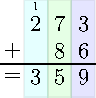
\includegraphics[]{rekfig/plus2}
	\end{figure}
}
}\\[12pt]
\parbox{0.3\linewidth}{
\eks[3]{
	\begin{figure}
		\centering
		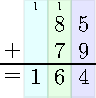
\includegraphics[]{rekfig/plus3}
	\end{figure}
}}\qquad
\parbox{0.3\linewidth}{
\eks[4]{
	\begin{figure}
		\centering
		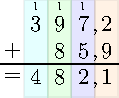
\includegraphics[]{rekfig/plus4}
	\end{figure}
}}
\end{center}
\fork{Eksempel 1}{
\begin{figure}
	\centering
	\subfloat[]{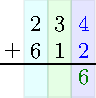
\includegraphics{rekfig/plus1a}}\qquad
	\subfloat[]{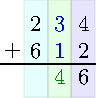
\includegraphics{rekfig/plus1b}}\qquad
	\subfloat[]{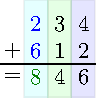
\includegraphics{rekfig/plus1c}}
\end{figure}

\begin{enumerate}[label=\alph*)]
	\item Vi legger sammen enerne: $ 4+2=6 $
	\item Vi legger sammen tierne: $ 3+1=4 $
	\item Vi legger sammen hundrene: $ 2+6=8 $
\end{enumerate}
} \newpage
\fork{Eksempel 2}{
	\begin{figure}
		\centering
		\subfloat[]{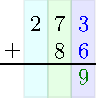
\includegraphics{rekfig/plus2a}}\qquad
		\subfloat[]{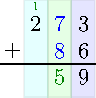
\includegraphics{rekfig/plus2b}}\qquad
		\subfloat[]{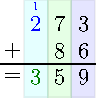
\includegraphics{rekfig/plus2c}}
	\end{figure}
	
	\begin{enumerate}[label=\alph*)]
		\item Vi legger sammen enerne: $ 3+6=9 $
		\item Vi legger sammen tierne: $ {7+8=15} $. Siden 10 tiere er det samme som 100, legger vi til 1 på hundreplassen, og skriver opp de resterende 5 tierne på tierplassen.
		\item Vi legger sammen hundrene: $ 1+2=3 $.
	\end{enumerate}
} \vsk

\spr{
Det å skrive 1 på neste sifferplass kalles ''å skrive 1 i mente''.
}
\begin{comment}
	\subsubsection{Tabellmetoden}
	Denne metoden tar utgangspunkt i det éne leddet, og summerer fram til det andre leddet er nådd. Det som i starten kan være litt rart med denne metoden, er at du selv velger fritt hvilke tall du skal legge til, så lenge du når det andre leddet til slutt.
	\begin{center}
		\parbox{0.3\linewidth}{
			\eks[1]{
				$ \colb{273}+\colc{86} = \colo{359} $ \vsk
				
				\begin{tabular}{r|r|r}
					&&\colb{273} \\ \hline
					6 & 6 & 279 \\
					30& 36 & 309 \\
					50& \colc{86} & \colo{359}
				\end{tabular}
			}
		} \qquad
		\parbox{0.3\linewidth}{
			\eks[2]{
				$ \colb{85}+\colc{79}=\colo{164} $  \vsk
				
				\begin{tabular}{r|r|r}
					& & \colb{85} \\ \hline 
					5 & 5 & 90 \\
					10 & 15 &100 \\
					64 & \colc{79} & \colo{164} \\
				\end{tabular} \vsk
			}
		}
	\end{center}
	\newpage
	\fork{Eksempel 1}{
		\begin{figure}
			\centering
			\subfloat[]{
				\begin{tabular}{r|r|r}
					&&\colb{273} \\ \hline
					&  &  \\
					\phantom{30}& \phantom{36} &  \\
					&  & 
				\end{tabular}
			} \qquad
			\subfloat[]{
				\begin{tabular}{r|r|r}
					&&\colb{273} \\ \hline
					6& 6 & 279 \\
					\phantom{30}& \phantom{36} &  \\
					&  & 
				\end{tabular}
			}\vsk 
			
			\subfloat[]{
				\begin{tabular}{r|r|r}
					&&\colb{273} \\ \hline
					6& 6 & 279 \\
					30& 36 & 309  \\
					&  & 
				\end{tabular}
			}
			\qquad
			\subfloat[]{
				\begin{tabular}{r|r|r}
					&&\colb{273} \\ \hline
					6& 6 & 279 \\
					30& 36 & 309  \\
					50& \colc{86} & \colo{359}
				\end{tabular}
			}
		\end{figure}
		\begin{enumerate}[label=(\alph*)]
			\item Vi starter med det leddet vi selv ønsker, ofte er det lurt å starte med det største leddet.
			\item Vi legger til $ 6 $. Da har vi totalt lagt til $ 6 $, og videre er $ {273+6=279} $.
			\item Vi legger til 30. Da har vi totalt lagt til 36, og videre er $ 279+30=309 $.
			\item Vi legger til 50. Da har vi totalt lagt til 86, altså har vi nådd det andre leddet, og videre er $ 309+50=359 $.
		\end{enumerate}
	} \vsk
	
	\info{Oppstilling versus tabellmetoden}{
		Ved første øyekast kan kanskje tabellmetoden bare se ut som en innviklet måte å regne addisjon på samenlignet med oppstilling, men med øving vil mange oppdage at tabellmetoden bedrer evnen til hoderegning. Styrkene til tabellmetoden kommer aller best til sin rett når det er snakk om å utføre subtraksjon eller divisjon.
	}
\end{comment}

\section{Subtraksjon}
\subsubsection{Oppstilling}
Subtraksjon med oppstilling baserer seg på plassverdisystemet, der man trinnvis regner differansen mellom enerne, tierne, hundrene, o.l. Metoden tar også utgangspunkt i et mengdeperspektiv, og tillater derfor ikke differanser med negativ verdi (se forklaringen til \textsl{Eksempel 2}).
\begin{center}
	\parbox{0.3\linewidth}{
\eks[1]{
	\begin{figure}
		\centering
		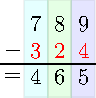
\includegraphics[]{rekfig/min1}
	\end{figure}
}} \qquad
\parbox{0.3\linewidth}{
\eks[2]{
	\begin{figure}
		\centering
		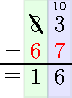
\includegraphics[]{rekfig/min2}
	\end{figure}
}} \\[12pt]
\parbox{0.3\linewidth}{
\eks[3]{
	\begin{figure}
		\centering
		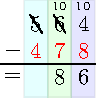
\includegraphics[]{rekfig/min3}
	\end{figure}
}}\qquad
\parbox{0.3\linewidth}{
\eks[4]{
	\begin{figure}
		\centering
		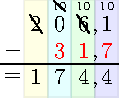
\includegraphics[]{rekfig/min4}
	\end{figure}
}}

\end{center}
\fork{Eksempel 1}{ \vs
\begin{figure}
	\centering
	\subfloat[]{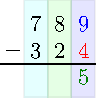
\includegraphics{rekfig/min1a}}\qquad
	\subfloat[]{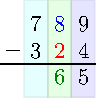
\includegraphics{rekfig/min1b}}\qquad
	\subfloat[]{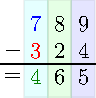
\includegraphics{rekfig/min1c}}
\end{figure}

\begin{enumerate}[label=(\alph*)]
	\item Vi finner differansen mellom enerne: $ {9-4=5} $
	\item Vi finner differansen mellom tierne: $ {8-2=6} $. 
	\item Vi finner differansen mellom hundrene: $ {7-3=4} $.
\end{enumerate}
}
\newpage
\fork{Eksempel 2}{ \vs
	\begin{figure}
		\centering
		\subfloat[]{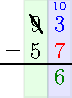
\includegraphics{rekfig/min2a}}\qquad
		\subfloat[]{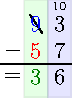
\includegraphics{rekfig/min2b}}
	\end{figure}
	
	\begin{enumerate}[label=(\alph*)]
		\item Vi merker oss at 7 er større enn 3, derfor tar vi 1 tier fra de 9 på tierplassen. Dette markerer vi ved å sette en strek over 9. Så finner vi differansen mellom enerne: $ {13-7=6} $
		\item Siden vi tok 1 fra de 9 tierne, er der nå bare 8 tiere. Vi finner differansen mellom tierne: $ {8-5=3} $.
	\end{enumerate}
}
\subsubsection{Tabellmetoden}
Tabellmetoden for subtraksjon tar utgangspunkt i at subtraksjon er en omvendt operasjon av addisjon. For eksempel, svaret på spørsmålet ''Hva er $ 789-324 $?'' er det samme som svaret på spørsmålet ''Hvor mye må jeg legge til på 324 for å få 789?''. Med tabellmetoden følger du ingen spesiell regel underveis, men velger selv tallene du mener passer best for å nå målet.\\
\begin{center}
\parbox{0.35\linewidth}{
\eks[1]{
$ \colb{789}-\colr{324}=\colc{465} $	 \vsk

\begin{tabular}{r|r}
	& \colr{324} \\ \hline
	6&330 \\
	70&400 \\
	389&\colb{789} \\ \hline
	\colc{465}
\end{tabular}
}} \qquad
\parbox{0.35\linewidth}{
	\eks[2]{
		$ \colb{83}-\colr{67}=\colc{16} $	 \vsk
		
		\begin{tabular}{r|r}
			& \colr{67} \\ \hline
			3&70 \\
			13&\colb{83} \\ \hline
			\colc{16}
		\end{tabular} \vspace{14pt}
}} \\[12pt]
\parbox{0.35\linewidth}{
	\eks[3]{
		$ 564-478=86 $\vsk
		
		\begin{tabular}{r|r}
			& 478 \\ \hline
			2&480 \\
			20&500 \\ 
			64&564\\ \hline
			86
		\end{tabular}
}} \qquad 
\parbox{0.4\linewidth}{
	\eks[4]{
		$ {206,1-31,7=174,4} $\vsk
		
		\begin{tabular}{r|r}
			& 31,7 \\ \hline
			0,3& 32\phantom{,0} \\
			70\phantom{,0}&102\phantom{,0} \\ 
			104,1&206,1\\ \hline
			174,4
		\end{tabular}
}}
\end{center}
\fork{Eksempel 1}{
	\[ \colb{789}-\colr{324}=\colo{465} \]
\begin{figure}
	\centering
	\subfloat[]{
	\begin{tabular}{r|r}
		& \colr{324} \\ \hline
		& \\
		& \\
		& \\ \hline
		&
	\end{tabular}	
} \qquad
	\subfloat[]{
	\begin{tabular}{r|r}
		& \colb{324} \\ \hline
	   \colb{6}& \colc{330}\\
		& \\
		& \\ \hline
		&
	\end{tabular}
}\qquad
	\subfloat[]{
	\begin{tabular}{r|r}
		& 324 \\ \hline
		6& \colb{330}\\
		\colb{70}& \colc{400} \\
		& \\ \hline
		&
	\end{tabular}	
}  \\[12pt]
\subfloat[]{
	\begin{tabular}{r|r}
		& 324 \\ \hline
		6& 330\\
		70& \colb{400} \\
		\colb{389}& \colc{789}\\ \hline
		&
	\end{tabular}	
}\qquad
\subfloat[]{
	\begin{tabular}{r|r}
		& 324 \\ \hline
		\colb{6}& 330\\
		\colb{70}& 400 \\
		\colb{389}& 789\\ \hline
		\colo{465}&
	\end{tabular}	
}
\end{figure}
\begin{enumerate}[label=(\alph*)]
	\item Vi starter med 324.
	\item Vi legger til 6, og får $ {324+6=330} $
	\item Vi legger til 70, og får $ {70+330=400} $
	\item Vi legger til 389, og får $ {389+400=789} $. Da er vi framme på 789.
	\item Vi summerer tallene vi har lagt til:  $ {6+70+389=465} $
\end{enumerate}
}
\section{Ganging} \label{rekGanging}
\subsubsection{Ganging med 10, 100, 1\,000 osv.}
\reg[Å gange heltall med 10, 100 osv. \label{gangheltallmed10100}]{
	\vs
	\begin{itemize}
		\item Når man ganger et heltall med 10, får man svaret ved å legge til sifferet 0 bak heltallet.
		\item Når man ganger et heltall med 100, får man svaret ved å legge til sifrene 00 bak heltallet.
		\item Det samme mønsteret gjelder for tallene 1\,000, 10\,000 osv.
	\end{itemize}
}
\eks[1]{\vsb \vsb
	\alg{
		6\cdot \colb{10} &= 6\colb{0}\vn
		79\cdot \colb{10} &= 79\colb{0} \vn
		802\cdot\colb{10}&=802\colb{0}
	}
}
\eks[2]{ \vsb \vsb
\alg{ 
6\cdot\colb{100} &= 6\colb{00} \vn
79\cdot\colb{100} &= 7\,9\colb{00} \vn
802\cdot\colb{100} &=80\,2\colb{00}
}
}
\eks[3]{ \vsb \vsb
\alg{ 
	6\cdot\colb{1\,000} &= 6\,\colb{000} \vn
	79\cdot\colb{10\,000} &= 79\colb{0\,000} \vn
	802\cdot\colb{100\,000} &=80\,2\colb{00\,000}
}
}
\newpage
\reg[Å gange desimaltall med 10, 100 osv. \label{gangdesmed10100}]{
	\vs
	\begin{itemize}
		\item Når man ganger et desimaltall med 10, får man svaret ved å flytte komma en plass til høgre.
		\item Når man ganger et heltall med 100, får man svaret ved å flytte komma to plasser til høgre.
		\item Det samme mønsteret gjelder for tallene 1\,000, 10\,000 osv.
	\end{itemize}
}
\eks[1]{\vsb \vsb
	\alg{
		7\colr{,}9\cdot 10 &= 79\colr{,}=79 \vn
		38\colr{,}02\cdot10&=380\colr{,}2 \vn
		0\colr{,}57\cdot 10 &=05\colr{,}7=5\colr{,}7 \vn
		0\colr{,}194\cdot 10&= 01\colr{,}94=1\colr{,}94
	}
}
\eks[2]{ \vsb \vsb
	\alg{
		7\colr{,}9\cdot 100 &= 790\colr{,}=790 \vn
		38\colr{,}02\cdot100&=3802\colr{,}=3\,802 \vn
		0\colr{,}57\cdot 100 &=057\colr{,}=57 \vn
		0\colr{,}194\cdot 100&= 019\colr{,}4=19\colr{,}4
	}
}
\eks[3]{ \vsb \vsb
	\alg{
	7\colr{,}9\cdot 1\,000 &= 7900\colr{,}=7\,900 \vn
	38\colr{,}02\cdot10\,000&=380020\colr{,}=380\,200 \vn
	0\colr{,}57\cdot 100\,000 &=57000\colr{,}=57\,000
}
}
\info{Merk}{
\hrs{gangheltallmed10100}{Regel} er bare et spesialtilfelle av \rref{gangdesmed10100}. For eksempel, å bruke \rref{gangheltallmed10100} på regnestykket $ {7\cdot 10} $ gir samme resultat som å bruke \rref{gangdesmed10100} på regnestykket $ {7,0\cdot 10} $. 
}
\newpage
\fork{Å gange tall med 10, 100 osv.}{
Titallsystemet baserer seg på grupper av ti, hundre, tusen osv., og tideler, hundredeler og tusendeler osv (se \rref{titalsys}). Når man ganger et tall med 10, vil alle enere i tallet bli til tiere, alle tiere bli til hundrere osv. Hvert siffer forskyves altså én plass mot venstre. Tilsvarende forskyves hvert siffer to plasser mot venstre når man ganger med 100, tre plasser når man ganger med 1\,000 osv.
}
\subsubsection{Utvidet form}
Ganging på utvidet form bruker vi for å regne multiplikasjon mellom flersifrede tall. Metoden baserer seg på distributiv lov (\rref{gangpar}). \regv
\eks[1]{ \vs
\begin{figure}
	\centering
	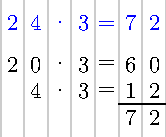
\includegraphics[]{rekfig/gang1}
\end{figure}
}
\eks[2]{ \vs
\begin{figure}
	\centering
	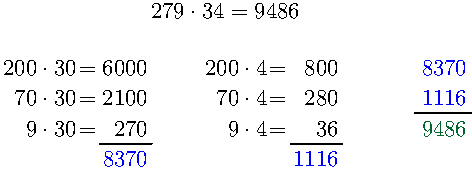
\includegraphics[]{rekfig/gfleirsif}
\end{figure}
}
\fork{Eksempel 1}{
24 kan skrives som $ 20+4 $, altså er
\[ 24\cdot3 =(20+4)\cdot3 \]
Av \rref{gangpar} har vi at 
\algv{
(20+4)\cdot 3 &=20\cdot 3 + 4\cdot 3 \\
&= 60+12 \\
&= 72
}
}
\newpage
\fork{Eksempel 2}{
Vi har at
\algv{
279&=200+70+9 \\
34 &=30+4 	
}
Altså er
\alg{
279\cdot34&= (200+70+9)\cdot (30+4) 
}
Videre er 
{
\footnotesize
\alg{
(200+70+9)\cdot (30+4) &=200\cdot 30+70\cdot30+9\cdot30+200\cdot4+70\cdot4+9\cdot4
\\
&=9486}
} \vs
}
\subsubsection{Kompaktmetoden}
Kompaktmetoden bygger på de samme prinsippene som ganging på utvidet form, men har en skrivemåte som gjør utregningen korterere. \regv

\eks[1]{
	\begin{figure}
		\centering
		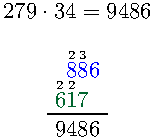
\includegraphics[]{rekfig/gfleirsifa}
	\end{figure}
}
\newpage
\fork{Eksempel 1}{
Vi starter med å gange sifrene i 279 enkeltvis med 4:
\begin{itemize}
	\item $ 9\cdot 6=36 $, da skriver vi 6 på enerplassen og 3 i mente.
	\item $ 7\cdot4 =28$, da skriver vi 8 på tierplassen og 2 i mente.
	\item $ 2\cdot 4=8 $, da skriver vi 8 på hundrerplassen.
\end{itemize}
Så ganger vi sifrene i 279 enkeltvis med 30. Dette kan forenkles til å gange med 3, så lenge vi plasserer sifrene én plass forskjøvet til venstre i forhold til da vi ganget med 4:
\begin{itemize}
	\item $ 9\cdot 3=27 $, da skriver vi 7 på tierplassen og 2 i mente. 
	\item $ 7\cdot3=21 $, da skriver vi 1 på hundrerplassen og 2 i mente.
	\item $ 2\cdot3=6 $, da skriver vi 6 på tusenplassen.
\end{itemize} 
}
\section{Divisjon} \label{rekDivisjon}
\subsubsection{\delmedtihundre}
\reg[Deling med 10, 100, 1\,000 osv. \label{deledesmed10100}]{
Når man deler et desimaltall med 10, får man svaret ved å flytte komma én plass til venstre.\vsk

Når man deler et desimaltall med 100, får man svaret ved å flytte komma to plasser til venstre.\vsk

Det samme mønsteret gjelder for tallene 1\,000, 10\,000 osv.
}
\eks[1]{ \vsb \vsb
	\alg{
200:10&=200\colr{,}0:10 \\&=20\colr{,}00\\&=20	\vn
45:10&=45\colr{,}0:10 \\&= 4\colr{,}50 \\&=4\colr{,}5
}
}
\eks[2]{ \vsb \vsb
	\alg{
		200:100&=200\colr{,}0:100 \\&=2\colr{,}000\\&=2	\vn
		45:100&=45\colr{,}0:100 \\&= 0\colr{,}450 \\&=0\colr{,}45
	}
}
\newpage
\eks[3]{ \vsb \vsb
\alg{
143\colr{,}7 :10 &= 14\colr{,}37 \vn
143\colr{,}7 :100 &= 1\colr{,}437 \vn
143\colr{,}7 :1\,000 &= 0\colr{,}1437 
}
}
\eks[4]{ \vsb \vsb
\alg{
93\colr{,}6:10 &= 9\colr{,}36 \vn
93\colr{,}6:100 &= 0\colr{,}936 \vn
93\colr{,}6:1\,000 &= 0\colr{,}0936
}
}
\fork{Deling med 10, 100, 1\,000 osv.}{
Titallsystemet baserer seg på grupper av ti, hundre, tusen osv., og tideler, hundredeler og tusendeler osv (se \rref{titalsys}). Når man deler et tall med 10, vil alle enere i tallet bli til tideler, alle tiere bli til enere osv. Hvert siffer forskyves altså én plass mot høgre. Tilsvarende forskyves hvert siffer to plasser mot høgre når man deler med 100, tre plasser når man deler med 1\,000 osv.
}

\subsubsection{Oppstilling}
Divisjon med oppstilling baserer seg på divisjon tolket som inndeling av mengder (se side \pageref{Divisjon})

\begin{center}
	\parbox{0.3\linewidth}{
	\eks[1]{ \vsb
		\begin{figure}
			\centering
			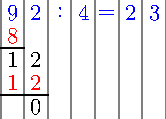
\includegraphics[]{rekfig/del1}
		\end{figure} \vspace{18pt}
	}
}\qquad
\parbox{0.45\linewidth}{
	\eks[1]{ \vspace{-5pt}
		\begin{figure}
			\centering
			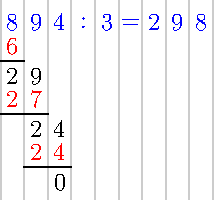
\includegraphics[]{rekfig/del2}
		\end{figure}
	}
}
\end{center}
\newpage
\fork{Eksempel 1}{ \vs \vs
	\begin{figure}
		\centering
		\subfloat{\includegraphics{\figp{delalg}}}
		\qquad \subfloat{\includegraphics[angle=90]{\figp{delalg0}}}
	\end{figure}
	Figuren over illustrerer mengden 92, som vi skal dele inn i 4 like store grupper. 
	\begin{itemize}
		\item Vi starter med å fordele så mange av tierne som mulig. Av de 9 tierne, kan hver gruppe få 2. Da har vi totalt fordelt $ 2\cdot 4=8 $ tiere.
		\begin{figure}
			\centering
			\subfloat{\includegraphics{\figp{delalgaa}}}
			\qquad \subfloat{\includegraphics[angle=90]{\figp{delalga}}}
		\end{figure}
		\item Vi står nå igjen med 1 tier og 2 enere, altså 12 enere. Av de 12 enerne, kan hver gruppe få 3. Da har vi totalt fordelt $ 3\cdot 4= 12 $ enere.
		\begin{figure}
			\centering
			\includegraphics[angle=90]{\figp{delalgb}}
		\end{figure}
		\item Nå er hele mengden 92 fordelt, og da er vi ferdige med utregningen. I hver gruppe endte vi opp med mengden 23.
	\end{itemize}
}
\newpage
\subsubsection{Tabellmetoden}
Tabellmetoden baserer seg på divisjon som omvendt operasjon av ganging. For eksempel er svaret på spørsmålet ''Hva er $ {76:4} $?'' det samme som svaret på spørsmålet ''Hvilket tall må jeg gange 4 med for å få 76?''. På samme vis som for tabellmetoden ved subtraksjon er det opp til en selv å velge passende tall for å nå målet.
\begin{center}
	\label{ekstbldiv}
	\parbox{0.35\linewidth}{
		\eks[1]{
			$ \colg{92}:\colb{4}=\colo{23} $	 \vsk
			
			\begin{tabular}{r|r|r}
				$ \cdot\, \colb{4} $&\\ \hline
				10&40&40 \\
				10&40&80 \\
				3& 12 &\colg{92} \\ \hline
				\colo{23}&
			\end{tabular}
			\vspace{28pt}
	}} \qquad
\parbox{0.35\linewidth}{
	\eks[2]{
		$ \colg{894}:\colb{3}=\colo{298} $	 \vsk
		
		\begin{tabular}{r|r|r}
			$ \cdot\, \colb{3} $&\\ \hline
			200& 600 &600 \\
			30&90 &690 \\
			30&90 &780 \\
			30& 90&870 \\
			8&24 &\colg{894} \\ \hline
			\colo{298} &
		\end{tabular}
}} \vsk

\parbox{0.415\linewidth}{
	\eks[3]{		
		$ 894:3=298 $	 \vsk
		
		\begin{tabular}{r|r|r}
			$ \cdot\, 3 $&\\ \hline
			300& 900&900 \\
			$ -2 $& $ -6 $ &894 \\ \hline
			298&
		\end{tabular} \vsk
	
\footnotesize	
\mer Samme regnestykke som i \textsl{Eksempel 2}, men en annen utregning.
}
}
\end{center}
\newpage
\fork{Eksempel 1}{
	Siden vi skal dele \colg{92} med \colb{4}, ganger vi med \colb{4} fram til vi når \colg{92}.
	\begin{figure}
		\centering
		\subfloat[]{
			\begin{tabular}{r|r|r}
				$ \cdot\, \colb{4} $&\\ \hline
				10&40&40 \\
				&& \\
				& &\\ \hline
				&
			\end{tabular}	
		} \qquad
		\subfloat[]{
			\begin{tabular}{r|r|r}
				$ \cdot\, \colb{4} $&\\ \hline
				10&40&40 \\
				10&40&80 \\
				&  & \\ \hline
				&
			\end{tabular}	
		} \\
		\subfloat[]{
			\begin{tabular}{r|r|r}
				$ \cdot\, \colb{4} $&\\ \hline
				10&40&40 \\
				10&40&80 \\
				3& 12 &\colg{92} \\ \hline
				&
			\end{tabular}	
		} \qquad
		\subfloat[]{
			\begin{tabular}{r|r|r}
				$ \cdot\, \colb{4} $&\\ \hline
				10&40&40 \\
				10&40&80 \\
				3& 12 &\colg{92} \\ \hline
				\colo{23}&
			\end{tabular}	
		}
	\end{figure}
	\begin{enumerate}[label=(\alph*)]
		\item Vi ganger 10 med 4, som er lik 40. Da har vi så langt kommet til 40.
		\item Vi ganger 10 med 4, som er lik 40. Da har vi så langt kommet til $ {40+40=80} $.
		\item Vi ganger 3 med 4, som er lik 12. Da har vi kommet til $ {80+12=92} $, som var målet.
		\item Vi legger sammen tallene vi ganget med, og får $ {10+10+3=23} $.
	\end{enumerate}
}
\info{Tips}{
	Det kan være lurt å se tilbake på utregninger gjort med tabellmetoden for å tenke over om man kunne valgt tall på en annen måte. I \textsl{Eksempel 1} på side \pageref{ekstbldiv} kunne vi startet med å gange med 20. Dette er omtrent like enkelt som å gange med 10, og det ville ha brakt oss nærmere målet.
}
\newpage
\subsubsection{Divisjon med rest}
Det er langt ifra alltid at svaret ved divisjon blir et heltall. En måte å uttrykke slike svar på, er å ved å bruke begrepet \outl{rest}\index{rest}. Begrepet er best forklart ved eksempel: \regv
\eks[1]{
	Regn ut $ 11:4 $ med rest.
	
	\sv
	Det største heltallet vi kan gange med 4 uten at produktet blir større enn
	11, er 2. $ {2\cdot 4 = 8} $, så da har vi $ 11-8=3 $ i rest.
	\[ 11= \colb{2}\cdot 4 +\colc{3} \]	
	\fig{mod1}
	Dette betyr at
	\[ 11:4 =\text{\colb{2} og \colc{3} i rest}\]
}
\eks[2]{
	Regn ut $ 19:3 $ med rest.
	
	\sv
	Det største heltallet vi kan gange med 3 uten at produktet blir større enn
	19, er 6. $ {6\cdot 3 = 18} $, så da har vi $ 19-8=1 $ i rest.
	\[ 19= \colb{6}\cdot 3 +\colc{1} \]	
	\fig{mod2}
	Dette betyr at
	\[ 19:3 =\text{\colb{6} og \colc{1} i rest}\]
}
\newpage
\eks[3]{
	Regn ut $ 94:4 $ med rest.
	
	\sv
	\metode{Med oppstilling}{3.75cm}
	\[ 94:4 = \text{23 og 2 i rest} \]
	\begin{figure}
		\centering
		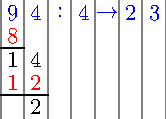
\includegraphics[]{rekfig/mod3}
	\end{figure}
	\mers{Da det blir feil å bruke \sym{$ = $} i figuren over, har vi valgt å bruke \sym{$  \rightarrow$}. 
	}\vsk 
	
	\metode{Med tabellmetoden}{3.75cm}
	\[ 94:4 = \text{23 og 2 i rest} \]
	\begin{center}
		\begin{tabular}{r|r|r}
			$ \cdot\, 4$&\\ \hline
			20&80&80 \\
			3& 12 &92 \\ \hline
			23&
		\end{tabular} \qquad $ 94-92=2 $
	\end{center}
}
\spr{
	Hvis vi utfører en \outl{modulo-operasjon}, finner vi resten i et delestykke. Dette blir ofte vist ved forkortingen \sym{mod}. For eksempel er
	\[ 11\text{ mod } 4= 3\qquad , \qquad 19\text{ mod 3} =1 \]
	I tillegg til \sym{\texttt{mod}}, blir også \sym{\texttt{\%}} og \sym{{\texttt{//}}} brukt som symbol for denne operasjonen i programmeringsspråk.
}
\newpage
\subsubsection{Divisjon med blanda tall som svar}
\eks[1]{
	Regn ut $ 11:4 $. Skriv svaret som et blandet tall.
	
	\sv \vsb
	\[ 11:4 = \text{2 og 3 i rest}=2+\frac{3}{4} \]
}
\eks[2]{
	Regn ut $ 19:3 $. Skriv svaret som et blandet tall.
	
	\sv \vsb
	\[ 19:3=\text{6 og 1 i rest}=6+\frac{1}{3} \]
}
\fork{Eksempel 1}{
	Vi starter med å legge merke til at $ 4=\frac{4}{1} $. Dette betyr at
	\[ 11:4 = 11:\frac{4}{1} \]
	Av \rref{delmbr} har vi at
	\[ 11:\frac{4}{1} = 11\cdot \frac{1}{4} \]
	Videre er $ 11=2\cdot 4+ 3 $, og da er
	\[ 11\cdot \frac{1}{4}=(2\cdot 4+3)\cdot\frac{1}{4} \]
	Av \rref{gangpar} har vi at
	\alg{
		(2\cdot 4+3)\cdot\frac{1}{4}&=2\cdot4\cdot\frac{1}{4}+3\cdot \frac{1}{4} \\
		&= 2+\frac{3}{4}
	}
}
\newpage
\subsection{Divisjon med desimaltall som svar}
\eks[1]{
	Regn ut $ 11:4 $. Oppgi svaret som desimaltal.
	
	\sv
	
	\metode{Med oppstilling}{3.75cm} \vs
	\[ 11:4=2,75 \]
	\begin{figure}
		\centering
		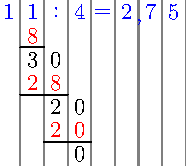
\includegraphics{rekfig/deldes1}
	\end{figure}
	\metode{Med tabellmetoden}{3.75cm} \vs
	\[ 11:4 = 2,75\]
	\begin{center}
		\begin{tabular}{r|r|r}
			$ \cdot\, 4$&\\ \hline
			2&8&8 \\
			0,5& 2 &10 \\
			0,25& 1 &11\\ \hline
			2,75&
		\end{tabular}
	\end{center}
}
\fork{Eksempel 1; oppstilling}{
	Siden vi deler med 4, er det snakk om å fordele 11 likt i 4 grupper.
	\begin{itemize}
		\item 8 av de 11 enerne kan vi fordele likt i 4 grupper. Da har vi igjen 3 enere. Dette er det samme som 30 tideler.
		\item 28 av de 30 tidelene kan vi fordele likt i 4 grupper. Da har vi igjen 2 tideler. Dette er det samme som 20 hundredeler.
		\item 20 av de 20 hundredelene kan vi fordele likt i 4 grupper.
		\item Hele mengden 11 er nå fordelt, og da er vi ferdige med utegningen.
	\end{itemize}
}
\newpage
\section{Regning med tid \label{regningmedtid}}
Sekunder, minutter og timer er organisert i grupper på 60:
\alg{
	1\text{ minutt} &= 60\text{ sekund} \\
	1\text{ time} &= 60\text{ minutt} 
}
Dette betyr at \textsl{overganger} oppstår i utregninger når vi når 60.\regv

\eks[1]{
	$ \text{2\enh{t} 25\enh{min} } + \text{10\enh{t} 45\enh{min}}= \text{13\enh{t} 10\enh{min} } $\vsk
	
	\metode{Utrekningsmetode 1}{0.35\linewidth}
	\os
	\begin{tabular}{r|r|r}
		& &10\enh{t} 45\enh{min}  \\ \hline
		15\enh{min}  &15\enh{min} & 11\enh{t} 00\enh{min}  \\
		10\enh{min} &25\enh{min} & 11\enh{t} 10\enh{min} \\
		2\enh{t} & 2\enh{t} 25\enh{min}  & 13\enh{t} 10\enh{min}
	\end{tabular} \vsk \vsk
	
	\metode{Utrekningsmetode 2}{0.35\linewidth}\os
	\begin{tabular}{r|r|r}
		& & 10:45 \\ \hline 
		00:15 & 00:15 & 11:00 \\
		00:10 & 00:25 & 11:10 \\
		02:00 & 02:25 & 13:10
	\end{tabular}
} \regv

\eks[2]{
	$ \text{14\enh{t} 18\enh{min} } - \text{9\enh{t} 34\enh{min}}= \text{4\enh{t} 44\enh{min} } $\vsk
	
	\begin{center}
		\parbox{0.4\linewidth}{
			\metode{Utrekningsmetode 1}{0.9\linewidth} \os
			\begin{tabular}{r|r}
				&  9\enh{t} 34\enh{min} \\ \hline 
				26\enh{min} & 10\enh{t} 00\enh{min} \\
				18\enh{min} & 10\enh{t} 18\enh{min} \\
				4\enh{t} & 14\enh{t} 00\enh{min} \\ \hline
				4\enh{t} 44\enh{min}
			\end{tabular}
		} \qquad \qquad
		\parbox{0.4\linewidth}{
			\metode{Utrekningsmetode 2}{0.9\linewidth} \os
			\begin{tabular}{r|r}
				& 09:34 \\ \hline 
				00:26 & 10:00 \\
				00:18& 10:18 \\
				04:00 & 14:18 \\ \hline
				04:44 
			\end{tabular}
		}
	\end{center}
}


\section{Avrunding og overslagsregning}

\subsubsection{Avrunding}
Ved \outl{avrunding} av et tall minker vi antall siffer forskjellige fra 0 i tallet. Videre kan man runde av til \textsl{nærmeste ener}, \textsl{nærmeste tier} og lignende.\regv
\eks[1]{
	Ved avrunding til \textsl{nærmeste tier} avrundes
	\begin{itemize}
		\item 1, 2, 3 og 4 \textsl{ned} til 0 fordi de er nærmere 0 enn 10.
		\item 6, 7, 8 og 9 \textsl{opp} til 10 fordi de er nærmere 10 \\enn 0.
	\end{itemize}	
	5 avrundes også opp til 10.
	\fig{avrnd0}
}

\eks[2]{ \vs
	\begin{itemize}
		\item $\boldmath \textbf{63 avrundet til nærmeste tier} = 60 $ \\
		Dette fordi 63 er nærmere 60 enn 70.
		\fig{avrnda}
		\item $\boldmath \textbf{78 avrundet til nærmeste tier} = 80 $ \\
		Dette fordi 78 er nærmere 80 enn 70.
		\fig{avrndb}
		\item $\boldmath \textbf{359 avrundet til nærmeste hundrer} = 400 $\\
		Dette fordi 359 er nærmere 400 enn 300.
		\fig{avrndc}
		\item $ \boldmath \textbf{11,8 avrundet til nærmeste ener} = 12$ \\
		Dette fordi 11,8 er nærmere 12 enn 11.
		\fig{avrndd}
	\end{itemize}
}

\subsection{Overslagsregning}
Det er ikke alltid vi trenger å vite svaret på regnestykker helt nøyaktig, ofte er det viktigere at vi fort kan avgjøre hva svaret \textsl{omtrent} er det samme som, aller helst ved hoderegning. Når vi finner svar som omtrent er riktige, sier vi at vi gjør et \outl{overslag}. Et overslag innebærer at vi avrunder\footnote{\textit{Obs!} Avrunding ved overslag trenger ikke å innebære avrunding til nærmeste tier og lignende.} tallene som inngår i et regnestykke slik at utregningen blir enklere. \vsk


\spr{
	At noe er ''omtrent det samme som'' skriver vi ofte som ''cirka'' (''ca.''). Tegnet for ''cirka'' er \sym{$ \approx $}.
} 

\subsubsection{Overslag ved addisjon og ganging}
La oss gjøre et overslag på regnestykket
\[ 98,2+24,6 \]
Vi ser at $ 98,2 \approx 100 $. Skriver vi 100 istedenfor 98,2 i regnestykket vårt, får vi noe som er litt mer enn det nøyaktige svaret. Skal vi endre på 24,6 bør vi derfor gjøre det til et tall som er litt mindre. 24,6 er ganske nærme 20, så vi kan skrive
\[ 98,2+24,6 \approx 100 + 20 = 120 \]
Når vi gjør overslag på tall som legges sammen, bør vi altså prøve å gjøre det ene tallet større (runde opp) og et tall mindre (runde ned).\\

\linje
Det samme gjelder også hvis vi har ganging, for eksempel
\[ 1\,689\cdot12 \]
Her avrunder vi 12 til 10. For å ''veie opp'' for at svaret da blir litt mindre enn det egentlige, avrunder vi 1\,689 opp til 1\,700. Da får vi
\[ 1\,689\cdot12\approx 1\,700\cdot 10 =17\,000 \]
\subsubsection{Overslag ved subtraskjon og deling}
Skal et tall trekkes fra et annet, blir det litt annerledes. La oss gjøre et overslag på
\[ 186,4-28,9 \]
Hvis vi runder 186,4 opp til 190 får vi et svar som er større enn det egentlige, derfor bør vi også trekke ifra noe. Det kan vi gjøre ved også å runde 28,9 oppover (til 30):
\alg{
	186,4-28,9&\approx 190-30 \\&=160
}
Samme prinsippet gjelder for deling: 
\[ 145:17 \]
Vi avrunder 17 opp til 20. Deler vi noe med 20 istedenfor 17, blir svaret mindre. Derfor bør vi også runde 145 oppover (til 150):
\[ 145:17 \approx 150:20 = 75 \]

\subsubsection{Overslagsregning oppsummert}
\reg[Overslagsregning \label{tipsoverslag}]{ \vs
	\begin{itemize}
		\item Ved addisjon eller multiplikasjon mellom to tall, avrund gjerne et tall opp og et tall ned.
		\item Ved subtraksjon eller deling mellom to tall, avrund gjerne begge tall ned eller begge tall opp.
	\end{itemize}	
}
\eks[]{
	Rund av og finn omtrentlig svar for regnestykkene.\os
	
	\abch{
		\item $ {23,1+174,7} $ 
		\item $ {11,8\cdot107,2} $ 		
	} \os
	\abchs{3}{
		\item $ {37,4-18,9} $  \ \ 
		\item $ {1054:209} $
	}
	\vspace{-2pt}
	
	\sv  \vspace{-7pt}
	\abc{
		\item $ 32,1 + 174,7 \approx 30+170 = 200 $
		\item $ 11,8 \cdot 107,2 \approx 10\cdot110 = 1\,100 $
		\item $ 37,4 - 18,9 \approx 40-20 = 20 $
		\item $ 1\,054:209 \approx 1\,000:200 = 5 $
	}
} \vsk

\info{Kommentar
}{
	Det finnes ingen konkrete regler for hva man \textsl{kan} eller ikke \textsl{kan} tillate seg av forenklinger når man gjør et overslag, det som er kalt \rref{tipsoverslag} er strengt tatt ikke en regel, men et nyttig tips.\vsk
	
	Man kan også spørre seg hvor langt unna det faktiske svaret man kan tillate seg å være ved overslagsregning. Heller ikke dette er det noe fasitsvar på, men en grei føring er at overslaget og det faktiske svaret skal være av samme \outl{størrelsesorden}. Litt enkelt sagt betyr dette at hvis det faktiske svaret har med tusener å gjøre, bør også overslaget ha med tusener å gjøre. Mer nøyaktig sagt betyr det av det faktiske svaret og ditt overslag bør ha samme tierpotens når de er skrevet på standardform\footnote{Se \refsec{Standardform}}.
}
\newpage
\section{Standardform} \label{Standardform}
\textit{Obs! Denne seksjonen tar utgangspunkt i at leseren er kjent med potenser, som vi ser på i \refsec{Potensar}.}\vsk

Vi kan utnytte \rref{gangdesmed10100} og \rref{deledesmed10100}, og det vi kan om potenser, til å skrive tall på \outl{standardform}. \vsk

La oss se på tallet 6\,700. Av \rref{gangdesmed10100} vet vi at
\[ 6\,700=6,7\cdot1\,000 \]
Og siden $ 1000=10^3 $, er
\[ 6\,700=6,7\cdot1\,000=6,7\cdot 10^3 \]
\st{
	$ 6,7\cdot10^3 $ er 6\,700 skrevet på standardform fordi
	\begin{itemize}
		\item 6,7 er større eller lik 1 og mindre enn 10.
		\item $ 10^3 $ er en potens med grunntall 10 og eksponent 3, som er et heltall.
		\item 6,7 og $ 10^3 $ er ganget sammen.
	\end{itemize}
}
\linje \\[12pt]

La oss også se på tallet  0,093. Av \rref{deledesmed10100} har vi at
\[ 0,093=9,3: 100 \]
Men å dele med 100 er det samme som å gange med $ 10^{-2} $, altså er
\[ 0,093=9,3: 100=9,3\cdot10^{-2} \]
\st{
	$ 9,3\cdot10^{-2} $ er 0,093 skrevet på standardform fordi	
	\begin{itemize}
		\item 9,3 er større eller lik 1 og mindre enn 10.
		\item $ 10^{-2} $ er en potens med grunntall 10 og eksponent $ -2 $, som er et heltall.
		\item $ 9,3 $ og $ 10^{-2} $ er ganget sammen.
	\end{itemize} 
}
\reg[Standardform]{
	Et tall skrevet som
	\[ a\cdot 10^n \]
	hvor $ {1\leq|a|<10} $ og $ n $ er et heltall, er et tall skrevet på standardform.
}
\eks[1]{
	Skriv 980 på standardform.
	
	\sv \vsb
	\[ 980 = 9,8\cdot 10^2 \]
}
\eks[2]{
	Skriv 0,00671 på standardform.
	
	\sv \vsb
	\[ 0,00671 = 6,71\cdot 10^{-3} \]
}
\info{Tips}{
	For å skrive om tall på standardform kan du gjøre følgende:
	\begin{enumerate}
		\item Flytt komma slik at du får et tall som ligger mellom 0 og 10.
		\item Gang dette tallet med en tierpotens som har eksponent med tallverdi lik antallet plasser du flyttet komma. \qquad  Flyttet du komma mot venstre/høgre, er eksponenten positiv/negativ. 
	\end{enumerate}
}
\eks[3]{
	Skriv 9\,761\,432 på standardform.
	
	\sv \vs
	\begin{enumerate}
		\item 	Vi flytter komma 6 plasser til venstre, og får $ 9\colr{,}761432 $
		\item Vi ganger dette tallet med $ 10^6 $, og får at 
		\[ 9\,761\,432=9,761432\cdot 10^6 \] 
	\end{enumerate}
}
\newpage
\eks[4]{
	Skriv 0,00039 på standardform.
	
	\sv \vs
	\begin{enumerate}
		\item Vi flytter komma 4 plasser til høgre, og får $ 3,9 $.
		\item Vi ganger dette tallet med $ 10^{-4} $, og får at
		\[ 0,00039=3,9\cdot10^{-4} \]
	\end{enumerate}
}
\end{document}

